% 번역본 공통 서식. tectonic으로 컴파일.
\documentclass[11pt,a4paper]{article}
\usepackage{fontspec}
\usepackage{xeCJK}
\setCJKmainfont[BoldFont={Apple SD Gothic Neo Bold},ItalicFont={AppleMyungjo},ItalicFeatures={FakeSlant=0.18}]{AppleMyungjo}
\setCJKsansfont{Apple SD Gothic Neo}
\setCJKmonofont{Apple SD Gothic Neo}
\xeCJKsetup{CJKspace=true,CJKecglue={},xCJKecglue=false}
\usepackage{amsmath,amssymb,mathtools,bm}
\usepackage[margin=24mm]{geometry}
\usepackage{booktabs,tabularx,array,multirow}
\usepackage{graphicx}
\usepackage{enumitem}
\usepackage{xcolor}
\usepackage[hidelinks]{hyperref}
\linespread{1.3}
\setlength{\parskip}{0.35em}
\newcolumntype{Y}{>{\raggedright\arraybackslash}X}
\newcommand{\E}{\mathbb{E}}
\newcommand{\Var}{\operatorname{Var}}
\renewcommand{\P}{\mathbb{P}}
\newcommand{\Q}{\mathbb{Q}}
\newcommand{\dd}{\mathsf{d}}   % 왜곡 척도 d (원문 산세리프)
\newcommand{\ff}{\mathsf{f}}
\renewcommand{\gg}{\mathsf{g}}  % 주의: ≫ 는 \ggg 대신 \gg 사용 불가
\newcommand{\ttl}{\jmath}      % d-기울인 정보 ȷ
\newcommand{\iinf}{\imath}     % 정보 확률변수 ı
\newcommand{\onote}[1]{\footnote{[옮긴이] #1}}
\renewcommand{\figurename}{그림}
\renewcommand{\tablename}{표}
\renewcommand{\abstractname}{초록}

\usepackage{fancyhdr}
\pagestyle{fancy}\fancyhf{}
\fancyhead[L]{\small 과업 지향 원천 부호화의 모델 인지 율-왜곡 한계 (한국어 번역)}
\fancyhead[R]{\small arXiv:2602.12866v1}
\fancyfoot[C]{\small\thepage}
\renewcommand{\headrulewidth}{0.3pt}
\renewcommand{\thesection}{\Roman{section}}
\renewcommand{\thesubsection}{\Alph{subsection}}
\renewcommand{\refname}{참고문헌}
\newcommand{\I}{\mathcal{I}}
\newcommand{\Hh}{\mathcal{H}}
\newcommand{\Yt}{\tilde{Y}}
\newcommand{\Yh}{\hat{Y}}
\newcommand{\Ys}{\mathcal{Y}}
\newcommand{\EC}{\mathrm{E\&C}}
\newcommand{\CE}{\mathrm{C\&E}}

\begin{document}

\noindent\fbox{\parbox{\dimexpr\linewidth-2\fboxsep-2\fboxrule}{\small
\textbf{번역본 안내.}
이 문서는 A.~Enttsel, V.~Corlay, ``Model-Aware Rate--Distortion Limits for Task--Oriented Source Coding,''
arXiv:2602.12866v1 [cs.IT], 2026년 2월 13일(\url{https://arxiv.org/abs/2602.12866})을 한국어로 옮긴 것이다.
원문은 Creative Commons 저작자표시 4.0 국제 라이선스(CC BY 4.0, \url{https://creativecommons.org/licenses/by/4.0/})로 공개되었고, 이 번역본도 같은 조건을 따른다.
변경 사항: 본문·캡션·각주·부록을 한국어로 옮겼고, 수식과 표는 다시 조판했으며, 그림은 원문에서 잘라 실었다. 참고문헌은 원문 그대로 두었다.
``[옮긴이]''로 시작하는 각주는 원문에 없는 번역자의 주석이다.
원저자는 이 번역을 검토하거나 보증하지 않았다. 인용할 때는 원문을 인용한다.
}}
\vspace{1em}

\begin{center}
{\Large\bfseries 과업 지향 원천 부호화의 모델 인지 율-왜곡 한계}\\[0.4em]
{\normalsize Model-Aware Rate--Distortion Limits for Task--Oriented Source Coding}\\[0.8em]
Andriy Enttsel, Vincent Corlay\\
Mitsubishi Electric R\&D Centre Europe, Rennes, France\\
\{a.enttsel, v.corlay\}@fr.merce.mee.com
\end{center}

\begin{abstract}
과업 지향 원천 부호화(TOSC, task-oriented source coding)는 기계 중심 추론 시스템에서 시각 데이터를 효율적으로 전달하는 패러다임으로 떠올랐다. 이런 시스템에서는 자원 제약 아래 비트율, 지연, 과업 성능을 함께 최적화해야 한다. 최근 연구들이 기계용 부호화의 율-왜곡 한계를 제시했지만, 이 결과들은 흔히 과업 식별 가능성에 대한 강한 가정에 기대며 실제로 배치된 과업 모델의 영향을 무시한다. 이 연구에서는 간접 율-왜곡 이론의 관점에서 단일 과업 TOSC의 근본 한계를 다시 살펴본다. 먼저 기존 율-왜곡 한계가 달성 가능한 조건을 밝히고, 현실적인 환경에서 그 한계가 어떻게 드러나는지 보인다. 이어서 과업 모델의 비최적성과 구조적 제약을 반영하는, 과업 모델을 인지하는 율-왜곡 한계를 도입한다. 표준 분류 벤치마크 실험에서 현재의 학습형 TOSC 방식이 이 한계에서 멀리 떨어져 동작함을 확인했으며, 이로부터 송신기 쪽 복잡도가 핵심 병목임을 알 수 있다.
\end{abstract}

\noindent\textbf{색인어}---과업 지향 원천 부호화, 기계용 부호화, 간접 율-왜곡 이론, 분류

\section{서론}
엣지 기기, 휴대전화, 자율주행차는 이미지, 동영상, 점군(point cloud)을 비롯한 막대한 양의 시각 데이터를 만들어 낸다. 많은 응용에서는 이 시각 콘텐츠를 처리해 의미 있는 정보를 뽑아내야 한다. 데이터의 규모를 고려하면, 오늘날 이 처리는 자동화되어 기계 분석 패러다임 아래 동작하는 비전 모델이 수행한다.

이를 위해 데이터는 흔히 압축되어, 계산 능력이 더 큰 클라우드로 보내진다. 기존의 원천 부호화는 원본 콘텐츠의 시각적(지각적) 충실도를 보존하는 것을 목표로 한다. 반면 기계용 부호화(CfM, coding for machines)라고도 하는 과업 지향 원천 부호화(TOSC)는 분류 [1], [2], 분할 [3], 객체 검출 [4]처럼 뒤따르는 과업의 정확도를 해치지 않으면서 데이터를 효율적으로 압축하는 것을 목표로 한다.

이와 관련된 틀로 인간-기계 협력 환경이 있다. 여기서는 코덱이 과업 성능과 시각 품질을 함께 최적화한다 [5]--[7]. 여러 과업을 대상으로 하는 환경도 연구되었다 [8], [9].

압축 성능을 특징짓는 두 가지 근본적인 양이 있다. 하나는 전달되는 정보의 양을 나타내는 율로, 시각 코덱에서는 보통 화소당 비트(bpp, bits per pixel)로 잰다. 다른 하나는 압축의 충실도로, 대개 과업에 맞는 적절한 왜곡 척도로 나타낸다. 율과 왜곡은 본질적으로 서로 경쟁하는 목표이며, 정보이론에서는 이 둘의 절충을 율-왜곡 함수 [10]로 정식화했다.

\paragraph{관련 연구}
이 연구에서는 최근 [11], [12]에서 다룬 단일 과업 지향 원천 부호화의 율-왜곡 분석을 더 발전시킨다. 신경망 기반 TOSC 시스템에서 흔한 패러다임은 특정 과업을 위해 설계한 모델(과업 모델)을 송신기와 수신기로 나누어, 과업 전단(front end)과 과업 후단(back end)을 정하는 것이다. 이 환경에서 전송 신호는 전단이 만든 중간 특징이다. 분할 지점은 근본적인 설계 선택이지만, [11]의 저자들은 정보이론 관점에서 이 선택이 최적 율-왜곡 성능에 영향을 주지 않음을 증명했다. 최적 성능은 과업과 그에 대응하는 왜곡 척도에만 달려 있다. 그런데도 [12]에서는 현재의 최신(SOTA, state-of-the-art) 단일 과업 TOSC 방식들이 일정 수준의 정확도를 얻는 데 필요한 비트율 면에서 이론적 한계와 몇 자릿수나 떨어져 동작함을 보였다. 그 주된 원인은 정보 병목 방법 [13]이 정보이론으로 정식화한, 무관한 정보 제거라는 개념과 연결되었다.

\paragraph{기여}
[12]에서 제안한 한계는 과업 관련 신호의 원천 부호화를 다루는 표준 율-왜곡 함수에서 유도되었다. 우리는 의미 통신의 율-왜곡에 관한 [14]의 연구, 특히 간접 율-왜곡 함수 [15], [16]를 바탕으로 다음을 수행한다. \emph{i}) [12]의 한계가 지니는 의미를 제한할 수 있는 암묵적 가정과 상황을 밝힌다. \emph{ii}) 과업에 의존할 뿐 아니라 과업 모델까지 명시적으로 반영하는 새로운 한계 세 가지를 제안한다. \emph{iii}) 최신 TOSC 방식을 제안한 한계와 비교해, 더 나은 성능에 이르는 데 가장 큰 병목이 송신기의 계산 복잡도와 구조적 복잡도 제약임을 밝힌다.

\section{단일 과업 TOSC의 율-왜곡 한계}
이 절에서는 \emph{간접 율-왜곡}(iRD, indirect rate--distortion) 이론 [15], [16]의 관점에서 단일 과업 TOSC의 근본 한계를 규명한다. 먼저 흔히 쓰이는 다른 율-왜곡 정식화와 대비해, iRD가 TOSC의 올바른 정보이론적 한계인 이유를 설명한다. 이어서 표준 부호화 전략이 iRD와 어떤 관계에 있는지, 어떤 가정 아래에서 최적일 수 있는지를 밝힌다.

이미지나 동영상 같은 관측 양식이 주어졌을 때, CfM과 TOSC의 목표는 과업 충실도 제약을 지키면서 가능한 가장 낮은 통신율로 과업 관련 잠재 변수(예: 클래스 레이블, 객체 정체)를 원격 에이전트에 전달하는 것이다.

신호의 흐름은 다음 마르코프 사슬로 나타낸다.
\begin{equation}
Y\to X\to \Yh,\tag{1}
\end{equation}
여기서 $Y$는 관측되지 않는 과업 관련 변수, $X$는 송신기에서 쓸 수 있는 관측, $\Yh$는 수신기에서 얻는 $Y$의 (왜곡되었을 수 있는) 복원이다. 채널 $Y\to X$는 데이터 생성 과정이 정하며 $p(x|y)$로 기술된다. 채널 $X\to\Yh$는 $p(\hat y|x)$로 기술되며 TOSC 설계가 정한다. (1) 아래에서 최적 율-왜곡 절충은 다음과 같다 [15], [16].
\begin{equation}
R_X(D_Y)=\min_{p(\hat y|x)}\I(X;\Yh)\quad\text{s.t.}\quad \E[d(Y,\Yh)]\le D_Y,\tag{iRD}
\end{equation}
여기서 상호 정보 $\I(X;\Yh)$는 통신율을 나타내고, $d(y,\hat y)$는 과업에 따른 왜곡 척도이다. 문제 (iRD)를 \emph{간접 율-왜곡 함수}(또는 원격 율-왜곡 함수, indirect or remote rate--distortion function)라고 하며, 단일 과업 TOSC의 진정한 근본 한계이다.

\subsection{분해형 부호화 전략에 의한 동작 한계}
(iRD)를 직접 푸는 것은 실제로는 대개 다루기 어렵다. 시각 콘텐츠를 나타내는 관측 $X$가 보통 고차원이고 복잡하기 때문이다. 그렇지만 설계를 분해형(factorized) 부호화 전략으로 제한하면 쓸모 있는 동작(operational) 한계를 얻을 수 있다. 이를 위해 $X\to\Yh$가 중간 표현 $Z$를 거쳐 분해되는, 더 일반적인 처리 사슬을 생각한다.
\begin{equation}
Y\to X\to Z\to\Yh.\tag{2}
\end{equation}
추가 처리를 송신기에서 하는지 수신기에서 하는지에 따라 두 가지 대표적인 TOSC 전략이 나온다.

\paragraph{1) 압축 후 추정}
압축 후 추정(C\&E, compress-and-estimate) 부호화 방식에서는 송신기가 먼저 관측 $X$를 압축해 $Z=\hat X$를 만들고, 이어서 수신기가 과업 변수를 $\Yh=g(\hat X)$로 추정한다(추정기 $g$를 흔히 과업 헤드라고 한다). 압축 단계는 고전적인(직접) 율-왜곡 함수 [17]로 기술된다.
\begin{equation}
R_X(D_X)=\min_{p(\hat x|x)}\I(X;\hat X)\quad\text{s.t.}\quad \E[d(X,\hat X)]\le D_X.\tag{RD}
\end{equation}
과업 왜곡은 $D_Y=\E[d(Y,g(\hat X))]$로 계산한다. C\&E는 과업과 무관할 수 있는 정보까지 포함해 관측 $X$ 전체를 전달하므로, 그 율-왜곡 성능은 (iRD)의 간접 율-왜곡 함수에 대한 \emph{달성 가능한 상한}이 된다. C\&E 전략은 $Y=X$인 퇴화한 경우에만 최적이며, 이때 (RD)는 (iRD)의 특수한 경우가 된다. 그렇지만 압축할 때 과업을 모르고 수신기에서야 과업이 정해지는 경우 [18]에는 C\&E가 의미가 있다. JPEG-AI 표준 [19]--[21]이 이 방향을 따른다.

\paragraph{2) 추정 후 압축}
추정 후 압축(E\&C, estimate-and-compress) 전략에서는 송신기가 먼저 과업 변수를 $Z=\Yt=f(X)$로 추정하고(추정기 $f$를 흔히 과업 모델이라고 한다) 그 추정값을 압축한다. 압축 단계는 추정한 변수에 대한 기존의 율-왜곡 함수로 기술된다.
\begin{equation}
R_{\Yt}(D_{\Yt})=\min_{p(\hat y|\tilde y)}\I(\Yt;\Yh)\quad\text{s.t.}\quad \E[d(\Yt,\Yh)]\le D_{\Yt}.\tag{eRD}
\end{equation}
이때 관련된 과업 왜곡은 $D_Y=\E[d(Y,\Yh)]$이다. E\&C는 원시 화소 영역의 관측 대신 과업과 관련된 표현을 압축하므로, 과업 추정이 충분히 정확하다면 같은 과업 왜곡에서 C\&E보다 낮은 율을 얻을 수 있다. E\&C가 최적인 대표적인 경우로, $X$와 $Y$가 결합 가우스이고 왜곡 $d(y,\hat y)$가 평균 제곱 오차(MSE, mean squared error)인 경우\footnote{이 경우 $f$는 최소 평균 제곱 오차 추정기이다.} [14], 그리고 압축이 무손실인 경우가 있다.

\subsection{식별 가능성과 오라클 율-왜곡 함수}
과업 변수가 송신기에서 완벽하게 \emph{식별 가능}(identifiable)하다고 가정하자. 즉 $Y=f(X)$인 결정론적 사상이 존재한다. 이는 조건부 엔트로피 $\Hh(Y|X)=0$과 같다. 이 경우 마르코프 사슬은 $X\to Y\to\Yh$로 줄어들고, (iRD)는 다음으로 단순해진다.
\begin{equation}
R_Y(D_Y)=\min_{p(\hat y|y)}\I(Y;\Yh)\quad\text{s.t.}\quad \E[d(Y,\Yh)]\le D_Y.\tag{oRD}
\end{equation}
이것은 과업 관련 변수의 기존 율-왜곡 함수이며, 우리는 이를 오라클 율-왜곡 함수(oRD, oracle rate--distortion function)라고 부른다. 이 함수는 $Y$의 손실 압축에 대한 \emph{절대 하한}이다.

정리하면 다음 부등식이 성립한다.
\begin{equation}
R_Y(D_Y)\le R_X(D_Y)\le\min\bigl\{R_X^{\CE}(D_Y),\ R_{\Yt}^{\EC}(D_Y)\bigr\},\tag{3}
\end{equation}
여기서 $R_X(D_Y)$는 (iRD)로 정의되고, 오른쪽 항들은 C\&E 전략과 E\&C 전략의 율-과업 왜곡 성능을 나타낸다.

식별 가능성 조건 $\Hh(Y|X)=0$은 최근 문헌 [11], [12]에서 흔히 암묵적으로 가정되지만, 강한 요구 조건이므로 주어진 과업마다 확인해야 한다. 잘 정제된 일부 벤치마크에서는 이 가정이 근사적으로 성립할 수 있지만, 잡음, 모호성, 내재적 불확실성이 있는 현실적인 시각 추론 상황에서는 자주 깨진다\footnote{이 측면은 부록에서 더 자세히 논의한다.}. 이 조건이 성립하지 않으면 한계 (oRD)는 일반적으로 \emph{달성할 수 없으며}(최적 추정기와 최적 압축기를 갖춘 완벽한 E\&C 전략으로도 그렇다), 진정한 TOSC 한계를 나타내지 못한다.

\subsection{동기를 주는 예}
완벽한 식별 가능성 아래에서 성립하는 한계 (oRD)가 도달 불가능하며 (iRD)보다 엄격하게 느슨할 수 있다는 점, 그리고 C\&E와 E\&C 어느 쪽도 일반적으로 TOSC에 최적이 아니라는 점을 보이기 위해, (1)의 다음 예를 생각한다. $Y$는 매개변수 $q=\P(Y=1)=0.5$인 $Y\sim\mathrm{Bernoulli}(q)$로 생성되고,
$Z\sim\mathcal N(0,1)$에 대해 $X=2Y-1+Z$이다. 그 결과 관측 $X$는 과업 관련 변수 $Y$를 이동시키고 가우스 잡음으로 오염시킨 것이 된다. $X$의 주변 밀도는 $p(x)=0.5p(x|y=0)+0.5p(x|y=1)=0.5\mathcal N(x;-1,1)+0.5\mathcal N(x;1,1)$로, 그림~1(왼쪽)에 보인 것처럼 두 성분이 같은 확률을 지니는 가우스 혼합 모델이다.

\begin{figure}[htbp]
\centering
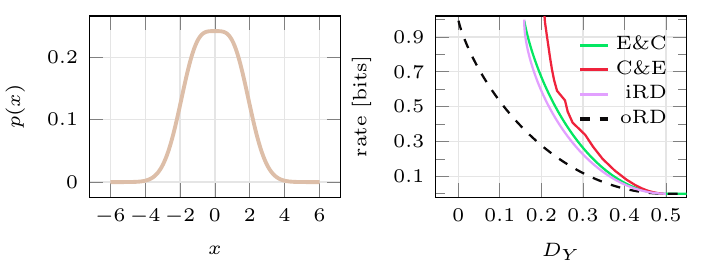
\includegraphics[width=0.75\linewidth]{fig/fig1.png}
\caption{클래스가 겹치는 가우스 혼합 모델: 확률 밀도(왼쪽)와 율-왜곡 성능(오른쪽).}
\label{fig:1}
\end{figure}

두 성분이 겹치므로 어떤 분류기도 두 성분을 완벽하게 구별해\footnote{이 경우 최대 사후 확률 결정 규칙으로 정의되는 최적 분류기는 부호를 판정한다: $f(X)=\mathrm{sign}(X)$.} $Y$를 식별할 수 없다. 그림~1(오른쪽)에서는 여러 TOSC 전략의 율-왜곡 성능을 비교한다. 이 원천에 대한 E\&C와 (iRD)는 [14]에서처럼 유도한다. 여기에 이진 원천에 맞춘 (oRD)와 C\&E 전략도 함께 나타냈다. C\&E 전략은 (RD)를 풀고 복원 $\hat x$에 최대 사후 확률(MAP, maximum a posteriori) 추정기를 적용한다(자세한 내용은 부록에 있다). 그림을 보면 완벽한 식별 가능성 가정은 최적 TOSC 성능에 대해 느슨하고 도달할 수 없는 하한을 주며, E\&C와 C\&E가 모두 최적이 아님을 알 수 있다.

\section{과업 모델에 의존하는 한계}
[12]에서 분석한 TOSC 한계는 오라클 율-왜곡 함수 (oRD)로 주어진다. 앞 절에서 논의했듯이 이 한계는 과업 관련 변수가 송신기에서 완벽하게 식별 가능하다는 가정에 기댄다. 게다가 (oRD)는 특정한, 그리고 최적이 아닐 수 있는 과업 모델을 쓴다는 실제적인 제약을 반영하지 않는다. 그런 과업 모델을 배치하면, 달성 가능한 율-왜곡 절충은 압축 전에 생기는 과업 모델 추정 오차
\begin{equation}
D_{\mathrm{TM}}=\E\Bigl[d\bigl(Y,\Yt\bigr)\Bigr]\tag{4}
\end{equation}
의 영향을 근본적으로 받는다.

이 연구에서는 대신 더 현실적인 간접 율-왜곡 함수 (iRD)를 직접 겨냥하면서 주어진 과업 모델을 명시적으로 반영하는 한계를 제안한다.

이 한계들 가운데 두 개는 E\&C 전략에 바탕을 둔다. 목표 왜곡이 더 줄일 수 없는 왜곡 바닥, 곧 $D_Y=D_{\mathrm{TM}}$과 같다면, E\&C 틀 안에서의 최적 전략은 $Y$를 추정한 뒤 그 추정값을 무손실로 압축하는 것이다. 추정값을 손실 압축하면 반드시 왜곡이 더해져 $D_Y>D_{\mathrm{TM}}$이 되기 때문이다. 더 큰 목표 왜곡 $D_Y>D_{\mathrm{TM}}$에 대해서는 (2)의 마르코프 사슬을 E\&C 경우로 특수화하자.
\begin{equation}
Y\to X\to\Yt\to\Yh.\tag{5}
\end{equation}
이 모델 아래에서는 추정기의 출력 $\Yt$를, 사상 $X\to\Yt$로 얻은 원격 원천 $Y$의 갱신된 관측으로 해석하면 $R_{\Yt}^{\EC}(D_Y)$를 곧바로 개선할 수 있다. 그러면 다음과 같은 적절한 간접 율-왜곡 함수가 나온다.
\begin{equation}
R_{\Yt}(D_Y)=\min_{p(\hat y|\tilde y)}\I(\Yt;\Yh)\quad\text{s.t.}\quad\E[d(Y,\Yh)]\le D_Y.\tag{iE\&C}
\end{equation}
이 정식화는 원천 $\Yt$가 주어졌을 때 E\&C를 개선하려면 압축기가 추정값 $\Yt$ 자체가 아니라 과업 관련 변수 $Y$를 복원해야 함을 시사한다. 우리는 이 방식을 간접 추정 후 압축(iE\&C, indirect estimate-and-compress)이라고 부른다. 추정과 압축은 여전히 분리되어 있지만, 압축은 과업 왜곡에 대해 직접 최적화된다. 실제로 iE\&C는 압축기가 더 효과적이려면 과업 레이블에 대해 학습되어야 한다는, 놀랍지 않은 사실로 이어진다\footnote{$Y$에 대한 지식은 학습 때에는 가정하지만 추론 때에는 가정하지 않는다.}.

iE\&C는 고정된 과업 모델로 제약된 설계 공간에서 고전적인 E\&C보다 엄격하게 더 촘촘한 기준을 주지만, 제약 없는 (iRD) 한계에 비하면 여전히 최적이 아니다.
\begin{equation}
R_Y(D_Y)\le R_X(D_Y)\le R_{\Yt}(D_Y)\le R_{\Yt}^{\EC}(D_Y).\tag{6}
\end{equation}

끝으로, (iRD)에 비해 iE\&C와 E\&C가 지니는 주된 장점은 고차원 원천 $X$에 대한 직접 최적화를 피하므로 실제로 계산할 수 있는 동작 한계라는 점이다.

\subsection{분류}
이제 분류 과업에 집중한다. 분류에서는 제안한 한계들을 Blahut--Arimoto(BA) 알고리즘 [17], [22]로 수치적으로 구할 수 있다. 표준 형태의 BA 알고리즘은 라그랑지안 완화 $R_Z+\lambda D_Z$를 풀어 이산 무기억 원천의 직접 율-왜곡 함수를 계산한다. 여기서 $Z\sim p(z)$는 이산 스칼라 확률변수이고, $\lambda>0$은 절충을 조절하는 라그랑주 승수이다.

분류에서 과업 관련 특징 $Y$는 알파벳 $\Ys=\{1,\dots,|\Ys|\}$ 위의 이산 확률변수이며, 사전 확률 $p(y)=\P(Y=y)$, $y\in\Ys$는 과업 데이터의 생성 과정이 암묵적으로 정한다. 추정기(분류 과업 모델)의 출력 $\Yt$도 같은 알파벳의 값을 취한다.

과업 모델을 학습하는 목표는 $X$에서 $\Yt$로 가는 사상을 학습해, $y,\tilde y\in\Ys$에 대한 조건부 분포 $p(\tilde y\mid y)=\P(\Yt=\tilde y\mid Y=y)$를 만들되, $d(\tilde y,y)=\mathbf 1\{\tilde y\ne y\}$일 때의 왜곡 $D_{\mathrm{TM}}=\E[d(Y,\Yt)]=\P(\Yt\ne Y)$를 최소화하는 것이다.

학습된 소프트맥스 기반 분류 과업 모델이 주어졌을 때, $f_{\mathrm{TM}}(x)\in\mathbb R^{|\Ys|}$를 소프트맥스 이전 층의 출력인 로짓 벡터라 하자. 이 모델은 다음과 같이 클래스 확률을 정의한다.
\begin{equation}
p(y\mid x)=\P(Y=y\mid X=x)=\mathrm{softmax}\bigl[f_{\mathrm{TM}}(x)\bigr]_y,\tag{7}
\end{equation}
그리고 대응하는 추정값 $\Yt$는 MAP 결정 규칙으로 얻는다. 이렇게 얻은 분류기는 혼동 행렬로 완전히 기술할 수 있으며, 행마다 정규화한 혼동 행렬은 채널 $p(\tilde y\mid y)$의 경험적 추정값이 된다. 예를 들어 이 분류기가 일으키는 왜곡과 주변 확률은 다음과 같이 계산할 수 있다.
\begin{align}
D_{\mathrm{TM}}=\P(\Yt\ne Y)&=\sum_{y\in\Ys}\P(\Yt\ne y\mid Y=y)\,p(y)\tag{8}\\
&=\sum_{y\in\Ys}\Bigl[1-\P(\Yt=y\mid Y=y)\Bigr]p(y)\tag{9}\\
p(\tilde y)=\P(\Yt=\tilde y)&=\sum_{y\in\Ys}p(\tilde y,y)=\sum_{y\in\Ys}p(\tilde y\mid y)\,p(y).\tag{10}
\end{align}

\paragraph{1) E\&C}
E\&C 전략에서는 (eRD)를 BA 알고리즘으로 수치적으로 풀 수 있다. BA 알고리즘은 $\tilde y\in\Ys$에 대한 $p(\tilde y)$를 입력으로 받아, $\lambda$와 왜곡 함수 $d(\tilde y,\hat y)=\mathbf 1\{\tilde y\ne\hat y\}$를 바탕으로 율, 왜곡, 그리고 채널
\begin{equation}
p(\hat y\mid\tilde y)=\P(\Yh=\hat y\mid\Yt=\tilde y)\tag{11}
\end{equation}
을 수치적으로 계산한다. 여기서 $\Yh$는 분류기 출력 $\Yt$의 복원을 나타내는 이산 확률변수이다. BA가 계산한 왜곡 $\E[d(\tilde y,\hat y)]$는 $p(\hat y\mid\tilde y)$를 통한 최적 손실 압축을 반영한다. 반면 $R_{\Yt}^{\EC}(D_Y)$를 평가하려면 다음 과업 왜곡 $D_Y$가 필요하다.
\begin{align}
D_Y=\E\Bigl[d(Y,\Yh)\Bigr]&=\P(\Yh\ne Y)\tag{12}\\
&=\sum_{y\in\Ys}\Bigl[1-\P(\Yh=y\mid Y=y)\Bigr]p(y).\tag{13}
\end{align}
(12)를 계산하려면 추정과 압축의 결합 효과를 담은 전체 채널 $p(\hat y\mid y)$를 평가해야 한다. (5)의 마르코프 사슬에서 $p(\hat y,\tilde y,y)=p(\hat y\mid\tilde y)\,p(\tilde y\mid y)\,p(y)$이므로, $Y$를 주변화하면 다음을 얻는다\onote{원문은 ``marginalizing out $Y$''라고 썼지만, 식 (14)에서 합으로 없애는 변수는 $\tilde Y$이다.}.
\begin{equation}
p(\hat y\mid y)=\sum_{\tilde y\in\Ys}p(\hat y\mid\tilde y)\,p(\tilde y\mid y).\tag{14}
\end{equation}

\paragraph{2) iE\&C}
(iE\&C)를 BA 알고리즘으로 풀려면, 과업 왜곡 $d(y,\hat y)$를 압축기가 보는 원천과 복원인 변수 $\Yt$와 $\Yh$로 나타내야 한다. 이는 조건부 기댓값 `기법' [16]으로 할 수 있다. 다음과 같은 유효 왜곡을 정의하면 충분하다.
\begin{equation}
\hat d(\tilde y,\hat y)=\E\Bigl[d(Y,\hat y)\mid\Yt=\tilde y\Bigr],\tag{15}
\end{equation}
그러면 전체 기댓값의 법칙에 따라 다음이 보장된다.
\begin{equation}
\E\Bigl[\hat d(\Yt,\Yh)\Bigr]=\E\Bigl[d(Y,\Yh)\Bigr]=D_Y.\tag{16}
\end{equation}
다시 말해 (15)의 왜곡을 입력으로 쓰면, BA 알고리즘은 기대 유효 왜곡을 최소화하고, 따라서 원래의 과업 왜곡을 최소화하는 것과 같다. 우리의 경우 조건부 기댓값의 정의에 따라 (15)를 닫힌 꼴로 나타낼 수 있다.
\begin{align}
\hat d(\tilde y,\hat y)&=\sum_{y\in\Ys}d(y,\hat y)\,p(y\mid\tilde y)=\sum_{y\in\Ys}\mathbf 1\{y\ne\hat y\}\,p(y\mid\tilde y)\tag{17}\\
&=1-\P(Y=\hat y\mid\Yt=\tilde y),\tag{18}
\end{align}
여기서 사후 확률은 다음과 같다.
\begin{equation}
p(y\mid\tilde y)=\P(Y=y\mid\Yt=\tilde y)=\frac{p(\tilde y\mid y)p(y)}{p(\tilde y)}.\tag{19}
\end{equation}

\paragraph{3) 표본 추출 후 전송}
iE\&C는 E\&C를 개선하지만, 일반적으로 TOSC의 최적 전략은 아니다. $D_Y>D_{\mathrm{TM}}$일 때, 최적의 분류 지향 부호화는 경판정 추정에 기대지 않고 과업 변수에 대한 연판정의, 곧 불확실성을 인지하는 표현을 활용한다는 것이 [14]에서 밝혀졌다. 이 표현은 (7)의 사후 확률 $p(y\mid x)$에 담기며, 과업 모델을 고정하면 이 사후 확률은 $Y$를 복원하기 위한 $X$의 베이즈 충분 통계량이다. 따라서 과업 모델로 제약된 최적 TOSC를 얻으려면, 경판정 추정값 $\Yt$가 아니라
\begin{equation}
V=\bigl(p(1\mid X),\dots,p(|\Ys|\mid X)\bigr)=\mathrm{softmax}[f_{\mathrm{TM}}(X)]\tag{20}
\end{equation}
에 대한 간접 율-왜곡 문제(TMRD라고 부른다)를 풀어야 한다.
\begin{equation}
R_V(D_Y)=\min_{p(\hat y|v)}\I(V;\Yh)\quad\text{s.t.}\quad\E[d(Y,\Yh)]\le D_Y.\tag{TMRD}
\end{equation}
안타깝게도 $V$는 연속값이고 고차원이어서 BA 알고리즘을 적용하기 어렵다. 그래서 우리는 이 통찰을 활용해, BA에 기대지 않으면서도 불확실성을 인지하는 표현의 이점을 담는 새로운 TOSC 한계를 정의한다.

(7)에 argmax 연산을 적용해 경판정 $\Yt$를 만든 뒤 압축하는 대신,
사후 확률에서 \emph{표본을 추출}한 뒤 그 표본을 수신기에 무손실로 \emph{전송}하는 상황을 생각한다. 그러면 복원을 다음과 같이 정의할 수 있다.
\begin{equation}
(\Yh\mid X=x)\sim\mathrm{Cat}\bigl(\mathrm{softmax}[\lambda f_{\mathrm{TM}}(x)]\bigr),\tag{21}
\end{equation}
여기서 Cat은 소프트맥스 출력을 매개변수로 하는 범주 분포이다. 역온도 매개변수 $\lambda$는 율-왜곡 절충을 발견법적으로 조절하려고 도입한 것이다.

동작 면에서 표본 추출 후 전송(S\&C, sample and communicate) 전략은 채널 시뮬레이션 [23], 또는 상대 엔트로피 부호화 [24]의 한 예이다. 채널 시뮬레이션에 관한 고전적 결과 [25]에 따르면, 필요한 통신율의 근본 한계는 $\I(X;\Yh)$로 주어진다.

S\&C 전략은 율 $\I(X;\Yh)$로 동작하므로 (iRD)가 정의하는 간접 율-왜곡 함수를 직접 겨냥하며, $\lambda$로 절충을 조절할 수 있다. 정성적으로 보면, $\lambda\to+\infty$일 때 소프트맥스 연산은 argmax처럼 동작하고 무손실 동작점을 되찾는다. $\lambda\to0$일 때는 표본 추출이 $X$와 독립인 $\Yh$를 만들어 두 변수 사이의 상호 정보를 최소화한다. 정량적으로는 주어진 데이터 집합 $\mathcal D=\{(x_i,y_i)\mid x_i\in\mathcal X,\ y_i\in\mathcal L\}$에서 $\I(X;\Yh)$와 $\E[d(Y,\Yh)]$를 경험적으로 추정해 율-왜곡 성능을 분석할 수 있다(자세한 내용은 부록에 있다).

그림~2에는 율-왜곡 동작을 정성적인 경향으로 요약했다. 고정된 과업 모델로 얻을 수 있는 최선의 율-왜곡 성능을 나타내는, 계산하기 어려운 (TMRD)와, TOSC의 근본 한계를 정하는, 역시 계산하기 어려운 (iRD)를 강조해 나타냈다. 한계 (TMRD)는 절대 하한 (oRD)와 여기서 다룬 과업 모델 의존 한계들의 하한(infimum) 사이에 있을 것으로 예상되며, (iRD)는 (oRD)와 (TMRD) 사이에 있다.

\begin{figure}[htbp]
\centering
\begin{minipage}[t]{0.3\linewidth}\centering
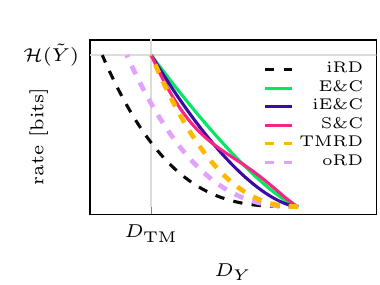
\includegraphics[width=\linewidth]{fig/fig2.png}
\caption{율-왜곡 한계의 정성적 동작.}
\label{fig:2}
\end{minipage}\hfill
\begin{minipage}[t]{0.67\linewidth}\centering
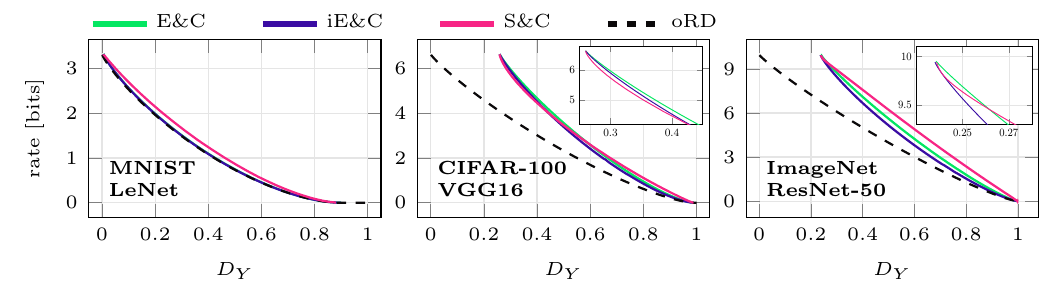
\includegraphics[width=\linewidth]{fig/fig3.png}
\caption{흔히 쓰이는 비전 과업 모델에 바탕을 둔, 표준 분류 벤치마크별 율-왜곡 성능.}
\label{fig:3}
\end{minipage}
\end{figure}

\subsection{일반화 가능성}
한계의 계산 방법은 대표적인 분류 문제에 대해 제시했지만, 그렇다고 이 틀의 적용 범위가 반드시 제한되는 것은 아니다. [12]에서 보였듯이 객체 검출 같은 과업은 이미지 안의 객체 위치와 객체 클래스의 여러 조합이 정하는 클래스들에 대한 분류로 바꿔 쓸 수 있으므로, 원리상 같은 율-왜곡 분석을 적용할 수 있다. 그 결과 생기는 제약은 개념적인 것이 아니라 계산상의 것이다. 이 점에서 S\&C의 장점은 클래스 수에 대해 선형으로 늘어난다는 것이다. 반면 BA는 제곱으로 늘어난다. 그렇지만 클래스 수가 많아 다른 방식들을 계산할 수 없을 때에는, (iRD)의 볼록성 덕분에 영율점 $(0,D_0)$과 무손실 추정점 $(\Hh(\Yt),D_{\mathrm{TM}})$을 잇는 간단한 아핀 상한\footnote{시분할(TS, time-sharing) 방식 [26, Ch.~8]으로 점근적으로 달성할 수 있다. 송신기는 확률 $\lambda$로 엔트로피 부호화한 추정값을 보내고, 확률 $1-\lambda$로 아무것도 보내지 않는다. 후자의 경우 수신기는 MAP에 따라 $\hat y=\arg\max_y p(y)$로 정한다. 스케줄링 규약을 양쪽이 알고 있으면 율은 $R=\lambda\Hh(\Yt)$, 왜곡은 $D_Y=\lambda D_{\mathrm{TM}}+(1-\lambda)D_0$이다.}을 쓸 수 있다. 여기서 $D_0=1-\max_y p(y)$이다.
\begin{equation}
R_{\Yt}^{\mathrm{TS}}(D_Y)=\frac{D_0-D_Y}{D_0-D_{\mathrm{TM}}}\Hh(\Yt)\quad\text{for}\quad D_{\mathrm{TM}}\le D_Y\le D_0.\tag{22}
\end{equation}

\section{수치 결과}
\subsection{율-왜곡}
앞에서 설명한 율-왜곡 한계를 보여 주기 위해 흔히 쓰이는 분류 벤치마크 세 가지, MNIST [27], CIFAR-100 [28], ImageNet [29]를 생각한다. MNIST에 대해서는 LeNet [30]에서 영감을 얻은 간단한 분류기를 설계했으며, 분류 정확도는 99.2\%이다($D_{\mathrm{TM}}=8\cdot10^{-3}$). CIFAR-100에 대해서는 미세 조정한 VGG-16 [31]을 써서 74\%의 분류 정확도를 얻었다($D_{\mathrm{TM}}=0.26$). ImageNet에 대해서는 76.1\%의 분류 정확도($D_{\mathrm{TM}}=0.239$)를 내는 ResNet-50 [32]을 배치했다. 그림~3에는 데이터 집합마다 E\&C, iE\&C, S\&C 기반 한계를 그렸다. 참고로 (oRD)에 해당하는 율-왜곡 곡선도 함께 그렸다. 모든 클래스 레이블이 균등 분포이므로 (oRD)에는 부록에 제시한 닫힌 꼴의 해가 있으며, 이는 [12]에서 분석한 한계에 해당한다. MNIST의 경우(그림~3 왼쪽) 거의 완벽한 판별은 E\&C와 iE\&C 전략이 (oRD)가 주는 절대 하한에 거의 도달함을 뜻한다. E\&C가 거의 최적이므로 S\&C를 포함한 다른 전략은 모두 최적이 아니다. 그림~3(가운데)의 CIFAR-100에서는 iE\&C가 언제나 E\&C보다 나으며, S\&C는 $0.26\le D_Y\le0.4$에서 iE\&C보다 나은 성능을 내고 $D_Y\ge0.57$에서는 E\&C보다 나빠진다. 끝으로 그림~3(오른쪽)에 나타낸 ImageNet에서는 iE\&C가 E\&C보다 상당히 개선되는 반면, S\&C는 $D_Y\simeq0.24$ 근처의 좁은 영역을 빼면 크게 최적에서 벗어난다.

강조하건대, S\&C는 사후 확률 표본 추출로 추정 불확실성을 반영하지만, 율-왜곡 절충을 오직 소프트맥스 온도 조절로만 제어한다. 이 방식에는 명시적인 최적성 보장이 없으며, 그래서 $D\gg D_{\mathrm{TM}}$에서 S\&C가 최적이 아니게 되는 것일 수 있다. 그렇지만 중요한 경험적 결과는 일부 상황에서 S\&C가 iE\&C보다 낫다는 것이다. 이는 iE\&C가 일반적으로 최적이 아님을 확인해 주며, 개선의 여지가 있음을 보여 준다.

끝으로 그림~4에서 정확도-화소당 비트(bpp)\footnote{bpp = 관측당 평균 비트율 / 화소 수} 곡선을 그려, 분류를 위한 현재의 SOTA ResNet-50 기반 TOSC 방식 [11]이 [12]에서 이미 관찰한 것처럼 도달 불가능한 한계 (oRD)에 비해 크게 최적에서 벗어날 뿐 아니라, 제안한 과업 모델 의존 한계에 비해서도 그렇다는 것을 보인다. 두 SOTA 곡선은 [11]의 율-정확도 분석에서 다룬 서로 다른 두 모델 분할 지점에 해당한다.

\subsection{복잡도}
추정기의 품질이 정확도를 제한하기는 하지만, 우리는 율의 격차가 주로 복잡도 제약 때문이라고 주장한다. 이 복잡도는 모델 크기를 비트로 재어 정량화한다\footnote{비트 단위 모델 크기는 디지털 객체의 복잡도에 대한 원리적인 정보이론적 개념인 Kolmogorov 복잡도 [33]의 거친 대리값이며, 모델 배치 벤치마크 [34]에서 널리 쓰인다.}.

제안한 한계는 크기 45.06\,MB\footnote{float 32 정밀도 대비 성능 손실이 없으므로 모델을 float 16 정밀도로 분석했다.}의 완전한 ResNet-50 모델이 송신기에서 동작한다고 가정한다. 송신기 쪽 복잡도 제약을 지키기 위해 SOTA1 방식은 Layer 4의 Block 0까지인 과업 전단만 배치하고\footnote{층 이름은 [11]의 관례를 따른다. 자세한 구조 그림은 해당 보충 자료의 Fig.~18을 보라.}, 완전 연결 층을 포함한 나머지 모델은 수신기에서 실행한다. 우리 분석에 따르면 이렇게 하면 송신기 쪽 모델 크기가 28\,MB로 거의 절반이 된다. SOTA2 구성은 Layer 3의 Block 4까지만 두어 크기를 12.16\,MB로 다시 절반 가까이 줄인다. 특징을 엔트로피 부호화하는 데 쓰는 추가 모델은 계산에 넣지 않았으므로, 실제 복잡도 감소는 이보다 작다.

이 주장을 더 뒷받침하기 위해, 그림~4에는 단순하지만 실제로 동작하는 단발(one-shot) TOSC 기준선의 성능을 하늘색으로 나타냈다. 구체적으로, 분류기 출력에서 얻은 주변 확률 $p(\tilde y)$가 가장 작은 $k$개 클래스를 기호 하나로 합치고, 그 기호를 $p(\tilde y)$가 가장 큰 클래스에 다시 배정해 축소된 코드북을 만든다. 이렇게 얻은 분포 $p(\tilde y)$를 엔트로피 부호화하며, 매개변수 $k$가 율-왜곡 절충을 조절한다. 제안한 한계와 비교하면, $\Yt$의 최적이 아닌 압축 때문에 생기는 율-왜곡\onote{원문은 ``rate---distortion''으로 대시 표기가 다른 곳과 다르다(오타로 보인다).} 비효율은 현재 SOTA 방식이 보이는 성능 격차에 비하면 무시할 만하다.

끝으로, 모델 분할과 직교하는 기법, 예컨대 가지치기와 양자화 [35], [36]\footnote{ResNet-50에 적용한 지도·비지도 가지치기 기법은 [36]의 보충 자료 Table~4를 보라.}를 써서 정확도 손실을 조금만 감수하고 송신기 쪽 복잡도를 줄일 수 있음을 밝혀 둔다.

\begin{figure}[htbp]
\centering
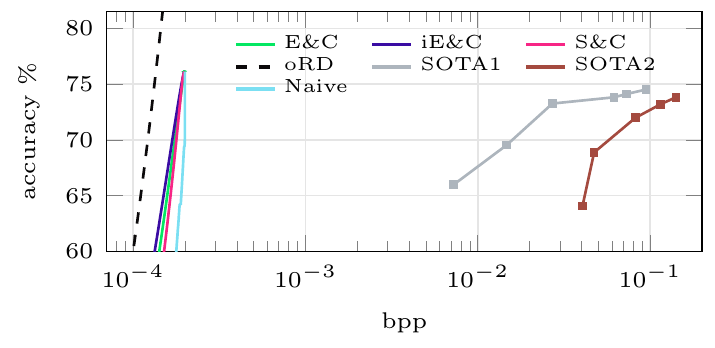
\includegraphics[width=0.62\linewidth]{fig/fig4.png}
\caption{최신 방식의 정확도 대 화소당 비트 성능을 이론적 한계 및 단순한 E\&C 기준선과 비교한 결과.}
\label{fig:4}
\end{figure}

\subsection{논의}
이 복잡도 고찰은 자원 제약 아래 과업 인지 압축에 관한 선행 연구와 일치한다. 예를 들어 [2], [9]의 저자들은 달성 가능한 율-정확도 절충이 엣지 모델의 복잡도 예산에 크게 좌우됨을 경험적으로 보였다. 그러나 그 연구들은 시스템과 학습의 관점을 택한 반면, 우리의 목표는 이 실제적인 한계를 근본적인 iRD 틀과 연결하고, 현재의 TOSC 방식이 정보이론 관점에서 본질적으로 최적이 아닌, 복잡도에 제한된 영역에서 동작함을 보이는 것이다.

[12]에서는 성능 격차를 현재 시스템에서 과업과 무관한 정보가 비효율적으로 제거되고 표현 학습이 최적이 아니라는 점과 연결하고, 정보 병목(IB) 원리 [13]를 사용했다. IB 정식화는 로그 손실 왜곡을 쓰는 iRD의 특수한 경우로 해석할 수 있다 [37]. 이 관점은 지금의 복잡도 분석과도 일치한다. 자원 제약 때문에 정보 병목이 처리 파이프라인의 너무 이른 곳에 사실상 삽입되고, 이것이 도달할 수 있는 율-왜곡 동작점을 제한해 iRD 한계와의 격차를 설명한다.

\section{결론}
이 연구에서는 간접 율-왜곡 이론의 관점에서 과업 지향 원천 부호화의 근본 한계를 다시 살펴보았다. 과업 모델의 비최적성을 명시적으로 반영해, 실제 TOSC 시스템에 동작 가능한 기준을 주는 모델 인지 율-왜곡 한계를 유도했다. 분석 결과 흔히 쓰이는 율-왜곡 한계는 현실적인 환경에서 성립하지 않을 수 있는 강한 식별 가능성 가정에 기댄다. 표준 분류 벤치마크에 대한 수치 결과는 현재의 최신 TOSC 방식이 이 한계에서 멀리 떨어져 동작하며, 송신기 쪽 복잡도와 그로 인한 모델 분할의 필요가 지배적인 병목으로 드러남을 보여 준다.

이 결과는 율-왜곡 분석만으로는 TOSC 성능을 충분히 평가할 수 없으며, 명시적인 복잡도 척도도 함께 고려해야 함을 확인해 준다. 추정 후 압축 전략은 일반적으로 최적이 아니지만, 율-왜곡 측면에서 여전히 실용적이며, 표준적인 모델 축소 기법과 함께 쓰면 원리상 실제 복잡도 제약을 충족할 수 있다.

\appendix
\renewcommand{\thesection}{}
\section*{부록}
\paragraph{표준 분류 벤치마크에서의 식별 가능성에 관한 논의}
문헌에서 흔히 쓰이는 오라클 율-왜곡 한계는 암묵적인 식별 가능성 가정 $\Hh(Y\mid X)=0$에 기댄다. 이 가정은 대부분의 비전 벤치마크가 사람이 레이블을 붙인 것이고, 각 이미지에 하나의 ``정답'' 레이블이 결정론적으로 배정된다는 사실에서 흔히 정당화된다.

그러나 사람의 주석이 정보이론적 의미의 식별 가능성을 뜻하지는 않는다. 더 충실하게 기술하면, 잠재 의미 변수 $Y$와, 관측 $X$에 작용하는 레이블링 과정이 만든 관측된 주석 $\Yt$를 구별해야 한다. 이로부터 다음 마르코프 사슬이 생긴다.
\begin{equation}
Y\to X\to\Yt,\tag{23}
\end{equation}
여기서 $\Yt$는 일반적으로 $Y$의 잡음 섞인 추정값이다. 주석 잡음이 작아 실제로 무시하더라도, 바탕에 있는 조건부 엔트로피 $\Hh(Y\mid X)$는 0이 되지 않는다.

더 나아가, 주석 잡음이 없더라도 데이터 획득이나 전처리 파이프라인의 비가역 변환 때문에 식별 가능성이 깨질 수 있다. 예를 들어 CIFAR-100 같은 저해상도 벤치마크에서는 다운샘플링 과정이 세밀한 시각 정보를 버리므로,
서로 다른 여러 의미 구성이 같은 관측 $X$를 낳을 수 있고, 이는 $\Hh(Y\mid X)>0$을 뜻한다. 이 현상은 표준 벤치마크의 오염된 판본에서 뚜렷해진다. 그런 판본에서는 잡음, 흐림, 그 밖의 섭동을 다양한 세기로 일부러 넣는다 [38].

이런 고찰에서 알 수 있듯이, 오라클 율-왜곡 한계의 바탕에 있는 식별 가능성 조건은 강한 모델링 가정이다. 이 가정은 정제된 데이터 집합에서는 근사적으로 성립할 수 있지만, 현실적인 시각 추론 상황에서는 일반적으로 깨진다. 그런 경우 오라클 율-왜곡 함수는 과업 지향 원천 부호화(TOSC)의 동작 한계를 나타내지 못하며, 간접 율-왜곡 정식화가 적절한 이론적 틀이 된다.

\paragraph{이진 원천의 율-왜곡 함수}
$Y\sim\mathrm{Bernoulli}(q)$에 대해 다음이 성립한다 [17, Th.~10.3.1].
\begin{equation*}
R_Y(D_Y)=\begin{cases}h(q)-h(D_Y), & 0\le D_Y\le\min(q,1-q)\text{일 때},\\ 0, & D_Y\ge\min(q,1-q)\text{일 때},\end{cases}
\end{equation*}
여기서 $h(u)=-u\log_2u-(1-u)\log_2(1-u)$는 이진 원천 $Z\sim\mathrm{Bernoulli}(u)$의 엔트로피이다.

\paragraph{C\&E 그래프의 세부 사항}
그림~1(오른쪽)의 C\&E 곡선을 그리기 위해, 먼저 원천을 이산화한 뒤 Blahut--Arimoto [22] 알고리즘을 적용해 율-왜곡 함수에 따른 채널 $p(\hat x\mid x)=\P(\hat X=\hat x\mid X=x)$를 계산한다. 복원된 표본이 주어졌을 때 최대 사후 확률 추정기에 바탕을 둔 최적 분류 규칙은 $\hat y=\arg\max_y p(y\mid\hat x)$와 $\P(\Yh=y\mid\hat X=\hat x)=\max_y p(y\mid\hat x)$를 준다. 그러면 과업 관련 왜곡은 다음과 같이 계산된다.
\begin{align*}
D_Y=\P(\Yh\ne Y)&=\sum_{\hat x}p(\hat x)\,\P(\Yh\ne Y\mid\hat x)\\
&=\sum_{\hat x}p(\hat x)\Bigl[1-\max_y p(y\mid\hat x)\Bigr],
\end{align*}
여기서 마르코프 사슬 $Y\to X\to\hat X$ 때문에 $p(y,x,\hat x)=p(\hat x\mid x)p(x\mid y)p(y)$이며, 사후 확률은 다음과 같이 계산한다\onote{마지막 분수의 합 첨자는 원문 그대로 $\hat x$이다. 앞 식과 맞추려면 분자·분모 모두 $\sum_x$여야 한다.}.
\begin{equation*}
p(y\mid\hat x)=\frac{p(y,\hat x)}{p(\hat x)}=\frac{\sum_x p(y,x,\hat x)}{p(\hat x)}=\frac{\sum_{\hat x}p(\hat x\mid x)p(x\mid y)p(y)}{\sum_{\hat x}p(\hat x\mid x)\,p(x)}.
\end{equation*}

\paragraph{S\&C의 추정 세부 사항}
상호 정보는 $\I(X;\Yh)=\Hh(\Yh)-\Hh(\Yh\mid X)$로 나타낼 수 있다. 먼저
\begin{equation*}
p(\hat y)\simeq\frac{1}{|\mathcal X|}\sum_{x_i\in\mathcal X}p(\hat y\mid x_i)
\end{equation*}
를 추정해 $\Yh$의 엔트로피
\begin{equation*}
\Hh(\Yh)=-\sum_{\hat y\in\hat{\Ys}}p(\hat y)\log_2p(\hat y)
\end{equation*}
를 계산한다. 조건부 엔트로피는 다음과 같이 추정한다.
\begin{align*}
\Hh(\Yh\mid X)&\simeq\frac{1}{|\mathcal X|}\sum_{x_i\in\mathcal X}\Hh(\Yh\mid X=x_i)\\
&=-\frac{1}{|\mathcal X|}\sum_{x_i\in\mathcal X}\Biggl\{\sum_{\hat y\in\hat{\Ys}}p(\hat y\mid x_i)\log_2p(\hat y\mid x_i)\Biggr\},
\end{align*}
왜곡을 계산할 때는 조건부 기댓값 $\E[d(Y,\Yh)]=\E[\hat d(X,Y)]$를 쓴다. 여기서
\begin{align*}
\hat d(x,y)=\E[d(\Yh,y)\mid X=x]&=\sum_{\hat y\in\hat{\Ys}}d(y,\hat y)\,p(\hat y\mid x)\\
&=\sum_{\hat y\in\hat{\Ys}}\mathbf 1\{y\ne\hat y\}\,p(\hat y\mid x)=1-\P(\Yh=y\mid X=x)
\end{align*}
이고, 경험적 추정값은 다음과 같다.
\begin{equation*}
\E[d(Y,\Yh)]\simeq1-\frac{1}{|\mathcal D|}\sum_{i=1}^{|\mathcal D|}\P(\Yh=y_i\mid X=x_i).
\end{equation*}

\paragraph{분류의 율-왜곡 함수}
$|\Ys|$개의 원소 $y\in\{1,\dots,|\Ys|\}$가 균등 분포인, 곧 모든 $y$에 대해 $p(y)=1/|\Ys|$인 이산 무기억 원천의 율-왜곡 함수는 다음과 같다.
\begin{equation*}
R_Y(D_Y)=\begin{cases}\log_2|\Ys|-h(D_Y)-D_Y\log_2(|\Ys|-1), & 0\le D_Y\le D_0\text{일 때},\\ 0, & D_Y\ge D_0\text{일 때},\end{cases}
\end{equation*}
여기서 $D_0=1-1/|\Ys|$이다.

\begin{thebibliography}{99}\small
\bibitem{b1} Saurabh Singh, Sami Abu-El-Haija, Nick Johnston, Jona Ballé, Abhinav Shrivastava, and George Toderici, ``End-to-end learning of compressible features,'' in \emph{Proc. IEEE Int. Conf. Image Process. (ICIP)}, 2020, pp.~3349--3353.
\bibitem{b2} Yoshitomo Matsubara, Ruihan Yang, Marco Levorato, and Stephan Mandt, ``Supervised compression for resource-constrained edge computing systems,'' in \emph{Proc. IEEE/CVF Winter Conf. Appl. Comput. Vis. (WACV)}, 2022, pp.~923--933.
\bibitem{b3} Nilesh Ahuja, Parual Datta, Bhavya Kanzariya, V. Srinivasa Somayazulu, and Omesh Tickoo, ``Neural rate estimator and unsupervised learning for efficient distributed image analytics in split-dnn models,'' in \emph{Proc. IEEE/CVF Conf. Comput. Vis. Pattern Recognit. (CVPR)}, 2023, pp.~2022--2030.
\bibitem{b4} Zhongzheng Yuan, Samyak Rawlekar, Siddharth Garg, Elza Erkip, and Yao Wang, ``Feature compression for rate constrained object detection on the edge,'' in \emph{Proc. IEEE Int. Conf. Multimedia Inf. Process. Retrieval (MIPR)}, 2022, pp.~1--6.
\bibitem{b5} Lingyu Duan, Jiaying Liu, Wenhan Yang, Tiejun Huang, and Wen Gao, ``Video coding for machines: A paradigm of collaborative compression and intelligent analytics,'' \emph{IEEE Trans. Image Process.}, vol.~29, pp.~8680--8695, 2020.
\bibitem{b6} Shuai Yang, Yueyu Hu, Wenhan Yang, Ling-Yu Duan, and Jiaying Liu, ``Towards coding for human and machine vision: Scalable face image coding,'' \emph{IEEE Trans. Multimedia}, vol.~23, pp.~2957--2971, 2021.
\bibitem{b7} Wenhan Yang, Haofeng Huang, Yueyu Hu, Ling-Yu Duan, and Jiaying Liu, ``Video coding for machines: Compact visual representation compression for intelligent collaborative analytics,'' \emph{IEEE Trans. Pattern Anal. Mach. Intell.}, vol.~46, no.~7, pp.~5174--5191, 2024.
\bibitem{b8} Saeed Ranjbar Alvar and Ivan V. Bajić, ``Pareto-optimal bit allocation for collaborative intelligence,'' \emph{IEEE Trans. Image Process.}, vol.~30, pp.~3348--3361, 2021.
\bibitem{b9} Yoshitomo Matsubara, Matteo Mendula, and Marco Levorato, ``A multi-task supervised compression model for split computing,'' in \emph{Proc. IEEE/CVF Winter Conf. Appl. Comput. Vis. (WACV)}, 2025, pp.~4913--4922.
\bibitem{b10} Toby Berger, \emph{Rate Distortion Theory: A Mathematical Basis for Data Compression}, Prentice Hall, Englewood Cliffs, NJ, 1971.
\bibitem{b11} Alon Harell, Yalda Foroutan, Nilesh Ahuja, Parual Datta, Bhavya Kanzariya, V. Srinivasa Somayazulu, Omesh Tickoo, Anderson de Andrade, and Ivan V. Bajić, ``Rate-distortion theory in coding for machines and its applications,'' \emph{IEEE Trans. Pattern Anal. Mach. Intell.}, vol.~47, no.~7, pp.~5501--5519, 2025.
\bibitem{b12} Ivan V. Bajić, ``Rate-accuracy bounds in visual coding for machines,'' in \emph{Proc. IEEE Int. Conf. Multimedia Inf. Process. Retrieval (MIPR)}, 2025, pp.~193--199.
\bibitem{b13} Naftali Tishby, Fernando C. Pereira, and William Bialek, ``The information bottleneck method,'' in \emph{Proc. Annu. Allerton Conf. Commun., Control, Comput.}, 1999, pp.~368--377.
\bibitem{b14} Jiakun Liu, Wenyi Zhang, and H. Vincent Poor, ``A rate-distortion framework for characterizing semantic information,'' in \emph{Proc. IEEE Int. Symp. Inf. Theory (ISIT)}, 2021, pp.~2894--2899.
\bibitem{b15} R. Dobrushin and B. Tsybakov, ``Information transmission with additional noise,'' \emph{IRE Trans. Inf. Theory}, vol.~8, no.~5, pp.~293--304, 1962.
\bibitem{b16} H. Witsenhausen, ``Indirect rate distortion problems,'' \emph{IEEE Trans. Inf. Theory}, vol.~26, no.~5, pp.~518--521, 1980.
\bibitem{b17} Thomas M. Cover and Joy A. Thomas, \emph{Elements of Information Theory}, Wiley, 2 edition, 2006.
\bibitem{b18} Alon Kipnis, Stefano Rini, and Andrea J. Goldsmith, ``The rate-distortion risk in estimation from compressed data,'' \emph{IEEE Trans. Inf. Theory}, vol.~67, no.~5, pp.~2910--2924, 2021.
\bibitem{b19} João Ascenso, Elena Alshina, and Touradj Ebrahimi, ``The jpeg ai standard: Providing efficient human and machine visual data consumption,'' \emph{IEEE MultiMedia}, vol.~30, no.~1, pp.~100--111, 2023.
\bibitem{b20} Elena Alshina, João Ascenso, and Touradj Ebrahimi, ``Jpeg ai: The first international standard for image coding based on an end-to-end learning-based approach,'' \emph{IEEE MultiMedia}, vol.~31, no.~4, pp.~60--69, 2024.
\bibitem{b21} Ayman Alkhateeb, Alessandro Gnutti, Fabrizio Guerrini, Riccardo Leonardi, João Ascenso, and Fernando Pereira, ``Jpeg ai compressed domain face detection: A multi-scale bridging perspective,'' \emph{IEEE Trans. Multimedia}, pp.~1--10, 2025.
\bibitem{b22} R. Blahut, ``Computation of channel capacity and rate-distortion functions,'' \emph{IEEE Trans. Inf. Theory}, vol.~18, no.~4, pp.~460--473, 1972.
\bibitem{b23} Cheuk Ting Li, ``Channel simulation: Theory and applications to lossy compression and differential privacy,'' \emph{Found. Trends Commun. Inf. Theory}, vol.~21, no.~6, pp.~847--1106, 2024.
\bibitem{b24} Gergely Flamich, Marton Havasi, and José Miguel Hernández-Lobato, ``Compressing images by encoding their latent representations with relative entropy coding,'' in \emph{Adv. Neural Inf. Process. Syst.}, 2020, vol.~33, pp.~16131--16141.
\bibitem{b25} C.H. Bennett, P.W. Shor, J.A. Smolin, and A.V. Thapliyal, ``Entanglement-assisted capacity of a quantum channel and the reverse shannon theorem,'' \emph{IEEE Trans. Inf. Theory}, vol.~48, no.~10, pp.~2637--2655, 2002.
\bibitem{b26} Raymond W. Yeung, \emph{Information Theory and Network Coding}, Information Technology: Transmission, Processing and Storage. Springer, New York, NY, 1 edition, 2008.
\bibitem{b27} Yann LeCun, Corinna Cortes, and Christopher J. C. Burges, ``The mnist database of handwritten digits,'' \url{http://yann.lecun.com/exdb/mnist/}, 1998.
\bibitem{b28} Alex Krizhevsky, Vinod Nair, and Geoffrey Hinton, ``Learning multiple layers of features from tiny images,'' Tech. Rep., University of Toronto, 2009.
\bibitem{b29} Olga Russakovsky, Jia Deng, Hao Su, Jonathan Krause, Sanjeev Satheesh, Sean Ma, Zhiheng Huang, Andrej Karpathy, Aditya Khosla, Michael Bernstein, Alexander C. Berg, and Li Fei-Fei, ``ImageNet Large Scale Visual Recognition Challenge,'' \emph{Int. J. Comput. Vis.}, vol.~115, no.~3, pp.~211--252, 2015.
\bibitem{b30} Y. Lecun, L. Bottou, Y. Bengio, and P. Haffner, ``Gradient-based learning applied to document recognition,'' \emph{Proc. IEEE}, vol.~86, no.~11, pp.~2278--2324, 1998.
\bibitem{b31} Karen Simonyan and Andrew Zisserman, ``Very deep convolutional networks for large-scale image recognition,'' \emph{arXiv preprint arXiv:1409.1556}, 2014.
\bibitem{b32} Kaiming He, Xiangyu Zhang, Shaoqing Ren, and Jian Sun, ``Deep residual learning for image recognition,'' in \emph{Proc. IEEE/CVF Conf. Comput. Vis. Pattern Recognit. (CVPR)}, 2016, pp.~770--778.
\bibitem{b33} Ming Li and Paul Vitányi, \emph{An Introduction to Kolmogorov Complexity and Its Applications}, Texts in Computer Science. Springer, Cham, 4 edition, 2019.
\bibitem{b34} Apple Inc., ``Optimizing resnet50 model,'' \url{https://apple.github.io/coremltools/docs-guides/source/opt-resnet.html\#id2}, 2024, Accessed: Jan. 22, 2026.
\bibitem{b35} Weihao Gao, Yu-Han Liu, Chong Wang, and Sewoong Oh, ``Rate distortion for model compression: From theory to practice,'' in \emph{Proc. Int. Conf. Mach. Learn. (ICML)}, 2019, pp.~2102--2111.
\bibitem{b36} Hongrong Cheng, Miao Zhang, and Javen Qinfeng Shi, ``A survey on deep neural network pruning: Taxonomy, comparison, analysis, and recommendations,'' \emph{IEEE Trans. Pattern Anal. Mach. Intell.}, vol.~46, no.~12, pp.~10558--10578, 2024.
\bibitem{b37} Deniz Gündüz, Zhijin Qin, Inaki Estella Aguerri, Harpreet S. Dhillon, Zhaohui Yang, Aylin Yener, Kai Kit Wong, and Chan-Byoung Chae, ``Beyond transmitting bits: Context, semantics, and task-oriented communications,'' \emph{IEEE J. Sel. Areas Commun.}, vol.~41, no.~1, pp.~5--41, 2023.
\bibitem{b38} Dan Hendrycks and Thomas Dietterich, ``Benchmarking neural network robustness to common corruptions and perturbations,'' in \emph{Int. Conf. Learn. Represent.}, 2019.
\end{thebibliography}


\end{document}
